En esta iteracion se implementara la opcion de anadir mas lugares al sistema, por lo que es necesario las consultas SQL que insertaran los datos enviados desde el dispositivo movil al servidor. \\

Como requisito para insertar un nuevo ``lugar'', se requiere que el usuario este posicionado en el ``lugar'' ya que se usaran sus coordenadas para posicionar el ``lugar''. Las coordenadas del usuario son obtenidas usuando el API de Geolocalizion propia de HTML5, usada anteriormente para encontrar la ubicacion del usuario \emph{visitante} en la iteracion 2.\\

Posteriormente se necesita implementar el formulario que el usuario usara para insertar los datos del ``lugar'': el nombre, la descripcion, el telefono y el nivel.\\

Para insertar un ``lugar''  en la base de datos se uso el codigo \ref{new_place}, donde se puede observar la consulta SQL usada, para la cual se necesita capturar la latitud y longitud respectiva donde se encuentra el usuario, ademas de los datos del ``lugar''.\\

\begin{center}
  \begin{lstlisting}[label=new_place,caption=Insertar un ``lugar'' en la base de datos.]

    var newPlace = (req, res) => {
        var name = req.body.name || '';
        var lat = req.body.lat || '';
        var lon = req.body.lon || '';
        var description = req.body.description || '';
        var phone = req.body.phone || '';
        var level = req.body.level || '';

        let raw = `insert into place (name, geom, description, phone, level)
                   values ('${name}',
                           ST_GeomFromText('POINT(${lon} ${lat})', 3875),
                           '${description}',
                           '${phone}',
                           '${level}'
                          );`;

        Knex.raw(raw)
            .then(function(data) {
                res.json({
                    "message": "Place saved successfully!",
                    "data": data
                });
            })
            .catch(function(error) {
                res.send("Error: ", error);
            });
    };

  \end{lstlisting}
\end{center}


Para la creacion de un ``lugar'' es necesario el implementar un \emph{endpoint} en el API y siguiendo las convenciones REST, para que como ya se explico anteriormente el frontend pueda comunicarse con el backend. \\


\begin{figure}[H]
      \begin{center}
        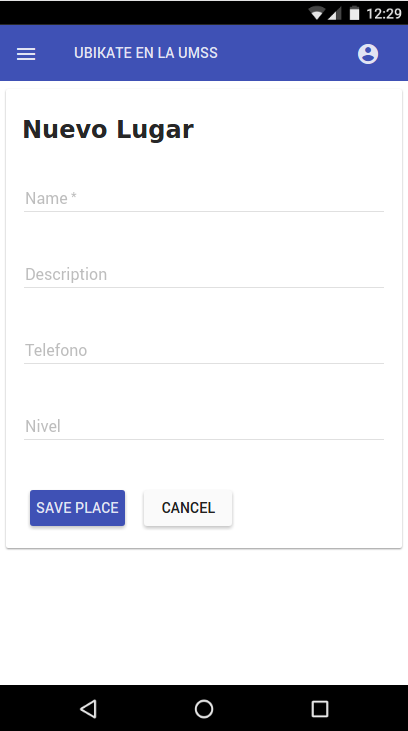
\includegraphics[width=0.45\textwidth]{new_place}

        % \caption{\emph{ember-leaflet} nos ayuda a desplegar un mapa y mostrar un \emph{punto} o \emph{lugar} con un \emph{marcador} y dibuja una línea de color rojo sobre el mapa.}
        \caption{ Formulario para anadir un nuevo ``lugar''}
        \label{fig:new_place}
        \caption*{Fuente: Elaboración propia.}
      \end{center}
\end{figure}
